\begin{figure}
	\centering
	\subfigure[$\Delta t$ = 1 día]{
	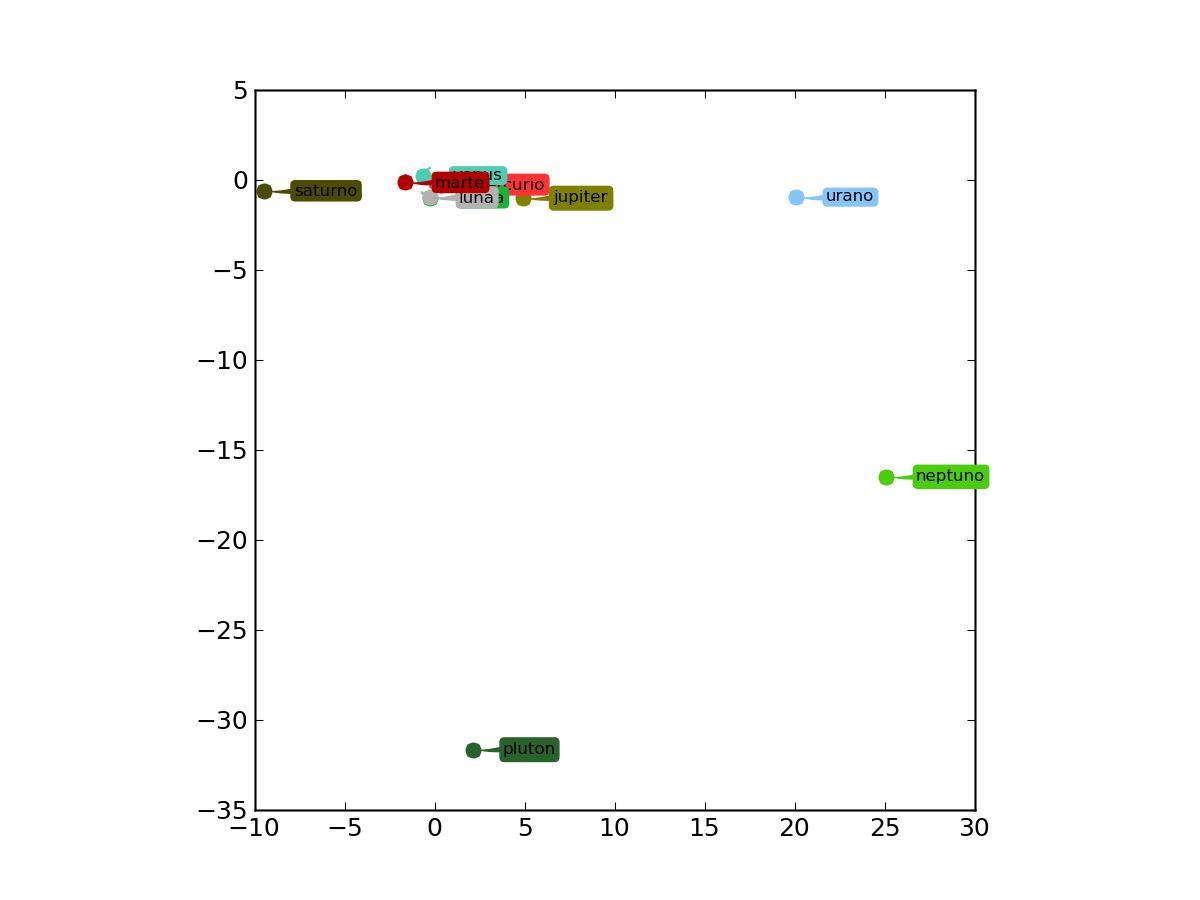
\includegraphics[scale=0.38]{img/ej2/metodo_1/validacion_30_1.png}
	\label{fig:ej2_m1_30_1}
	}
	\subfigure[$\Delta t$ = 6 horas]{
	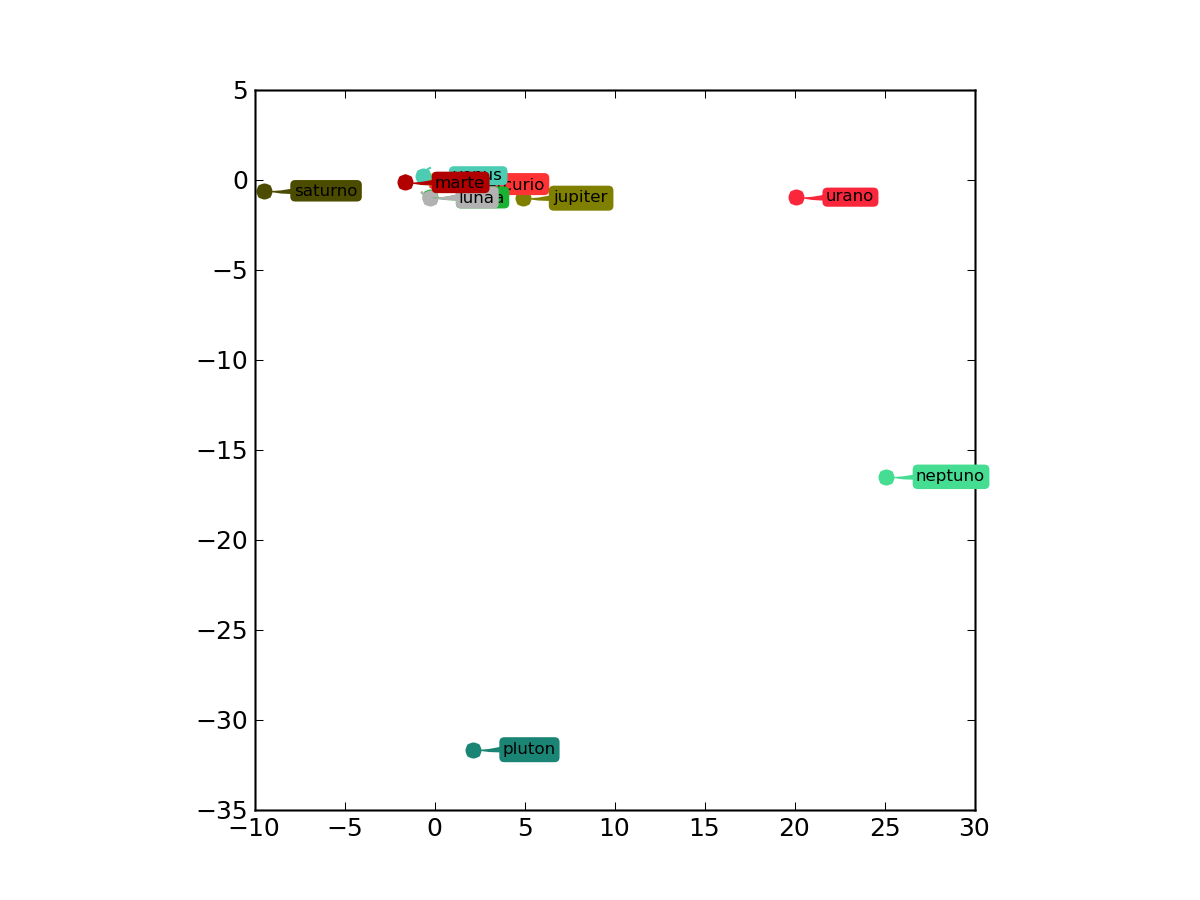
\includegraphics[scale=0.38]{img/ej2/metodo_1/validacion_30_4.png}
	\label{fig:ej2_m1_30_4}
	}
	\\
	\subfigure[$\Delta t$ = 2 horas]{
	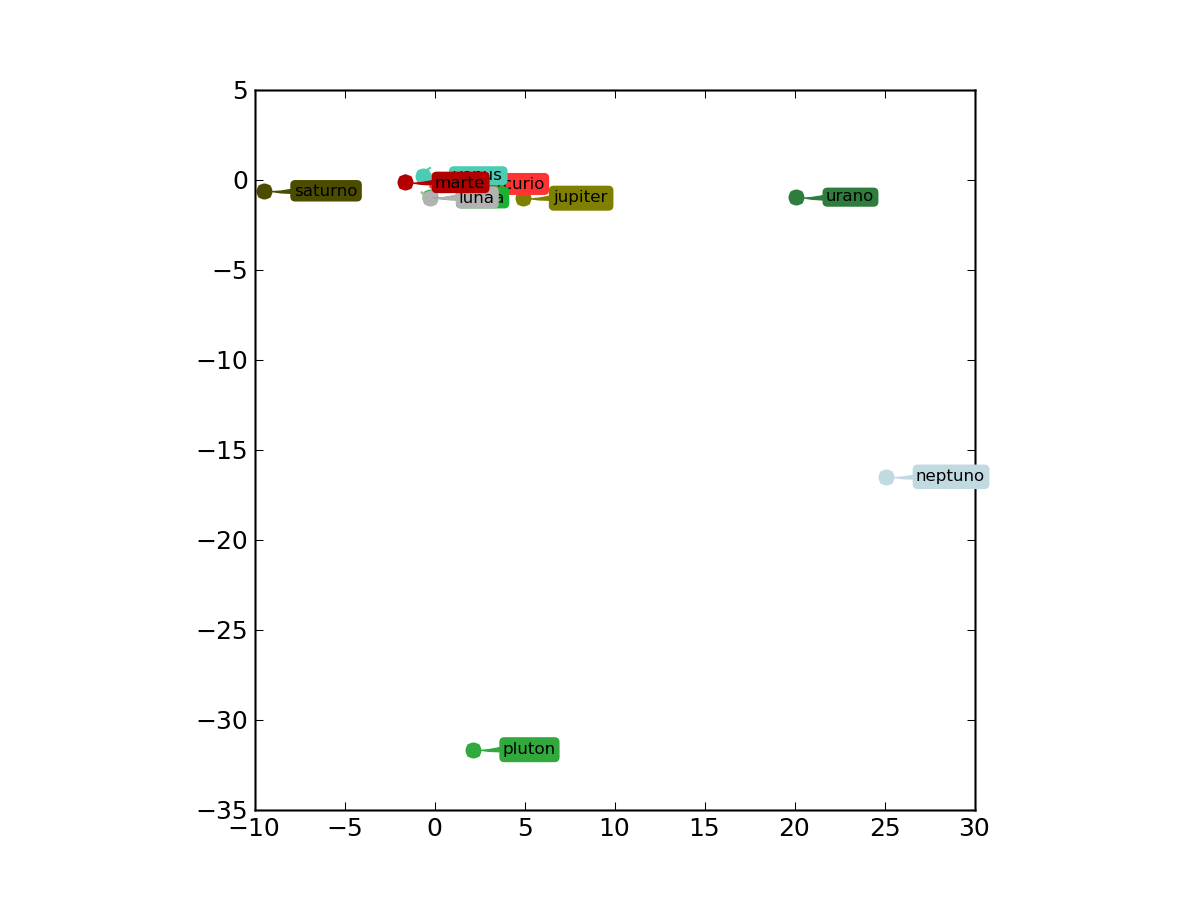
\includegraphics[scale=0.38]{img/ej2/metodo_1/validacion_30_12.png}
	\label{fig:ej2_m1_30_12}
	}
	\subfigure[$\Delta t$ = 1 hora]{
	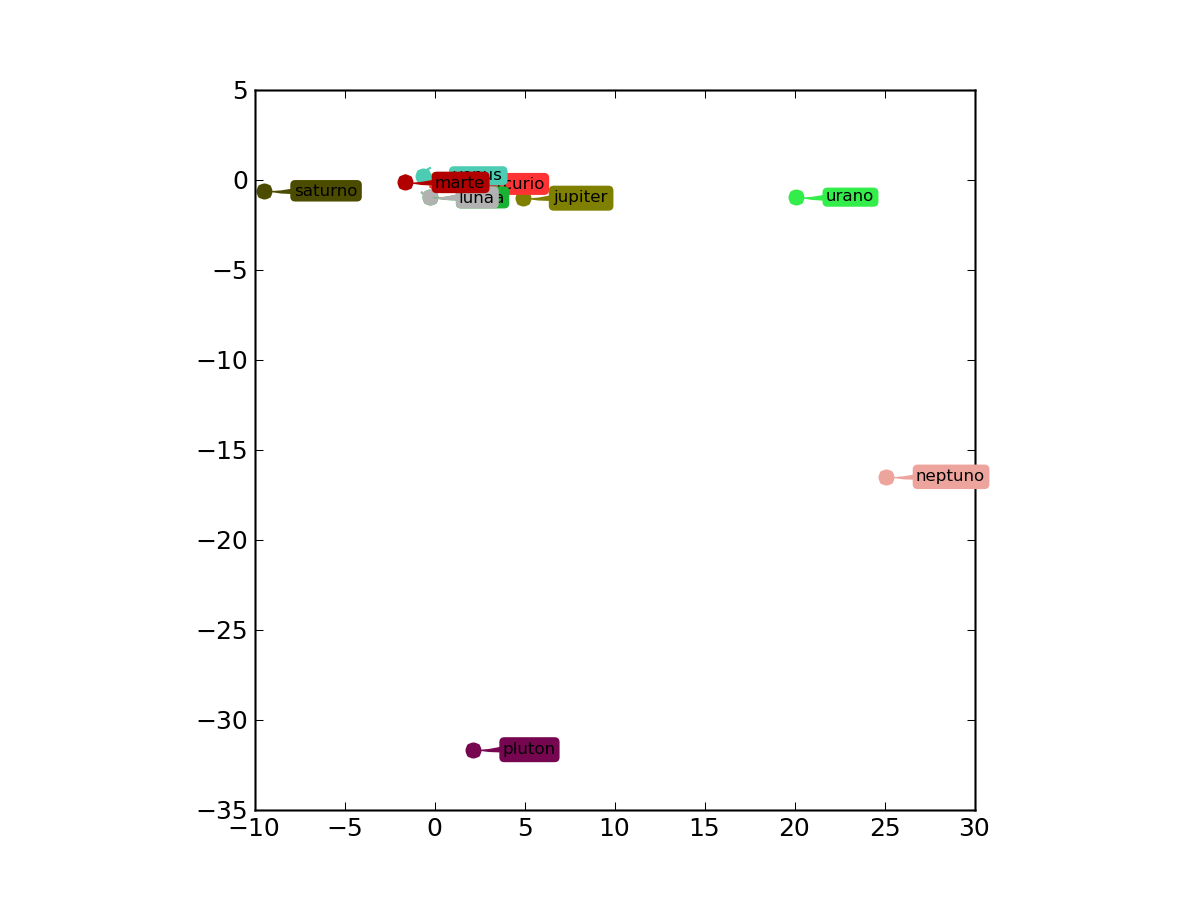
\includegraphics[scale=0.38]{img/ej2/metodo_1/validacion_30_24.png}
	\label{fig:ej2_m1_30_24}
	}
	\caption{
		Simulación de validación del sistema solar para un período de 30 días y distintos $\Delta t$
		con el método 1.
		No hay muchas observaciones que hacer ya que para las dimensiones del sistema solar en 30 días no cambia mucho.
	}
	\label{ fig:res_ej2_m1_30 }
\end{figure}
\begin{figure}
	\centering
	\subfigure[$\Delta t$ = 1 día]{
	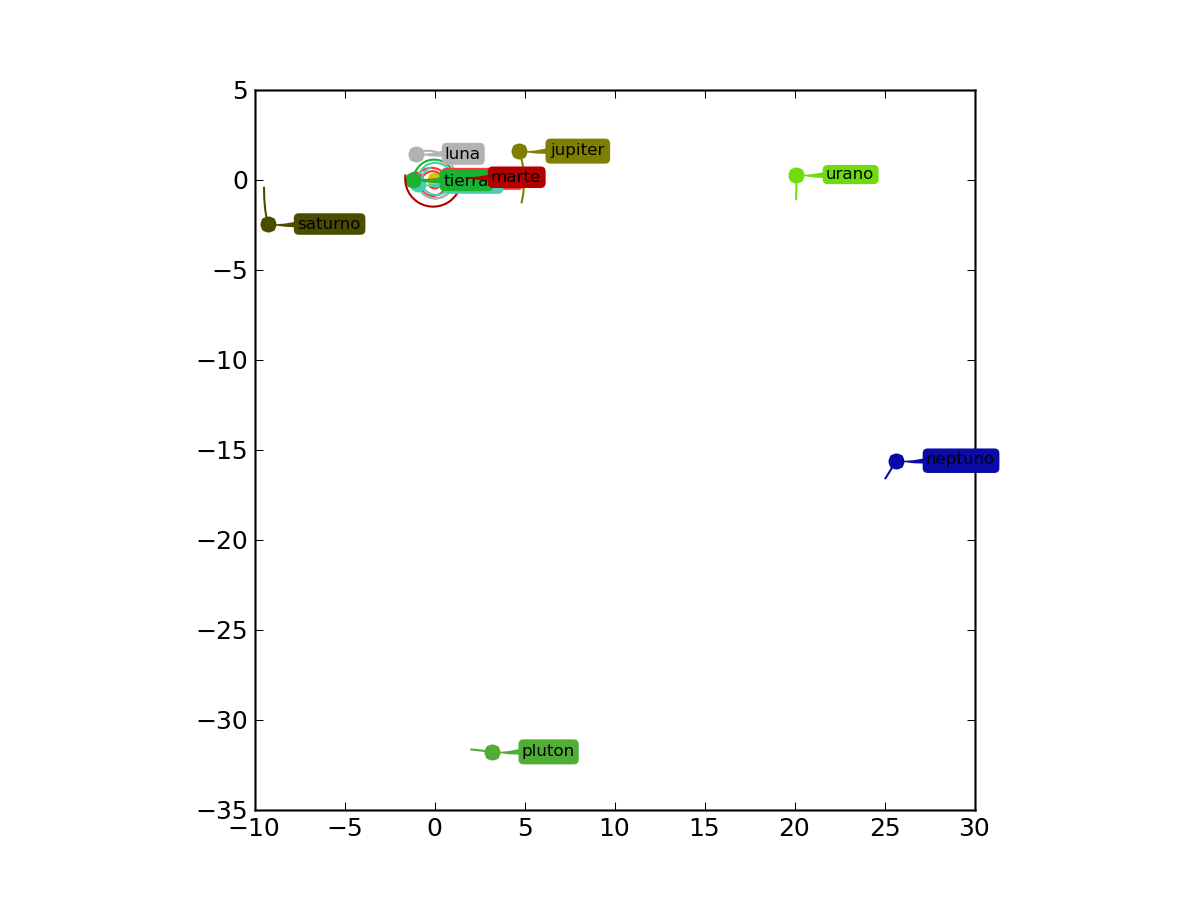
\includegraphics[scale=0.38]{img/ej2/metodo_1/validacion_365_1.png}
	\label{fig:ej2_m1_365_1}
	}
	\subfigure[$\Delta t$ = 6 horas]{
	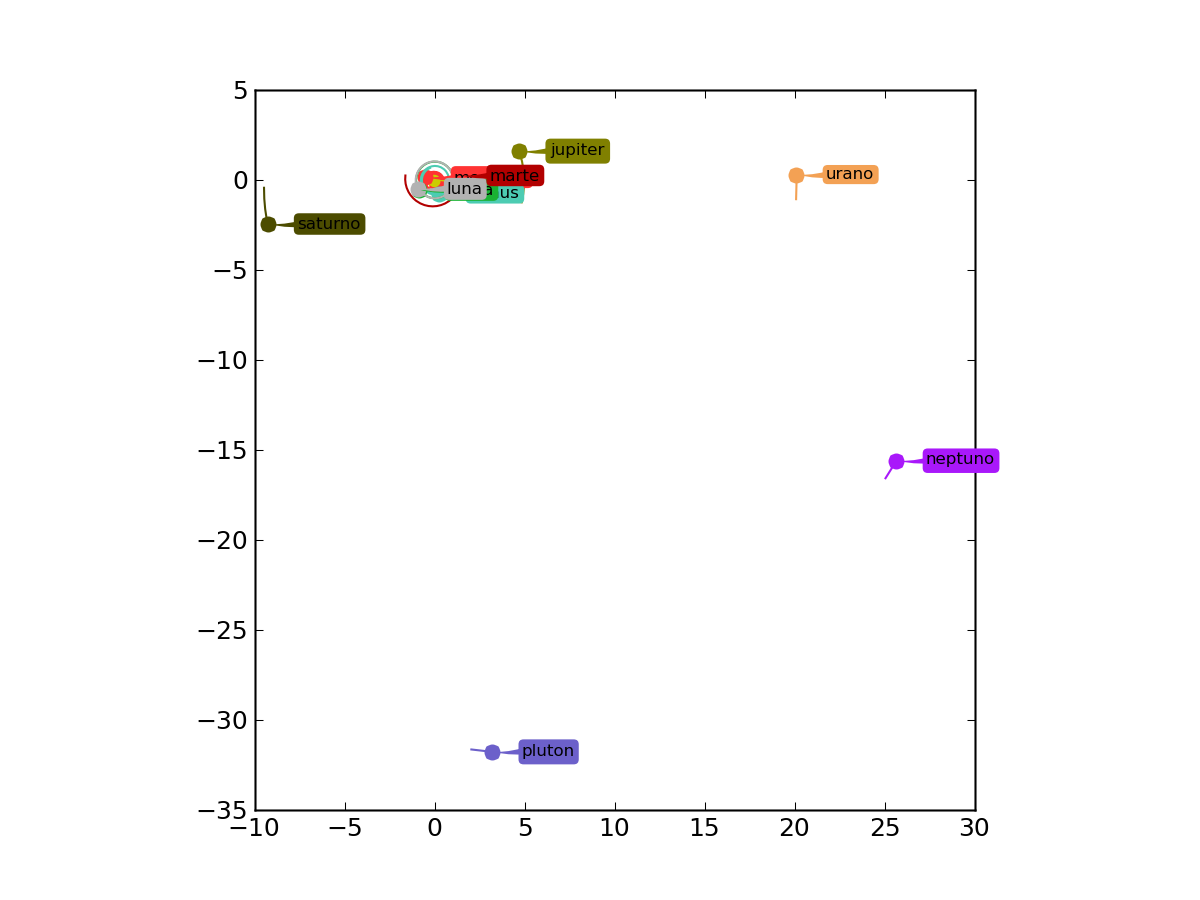
\includegraphics[scale=0.38]{img/ej2/metodo_1/validacion_365_4.png}
	\label{fig:ej2_m1_365_4}
	}
	\\
	\subfigure[$\Delta t$ = 2 horas]{
	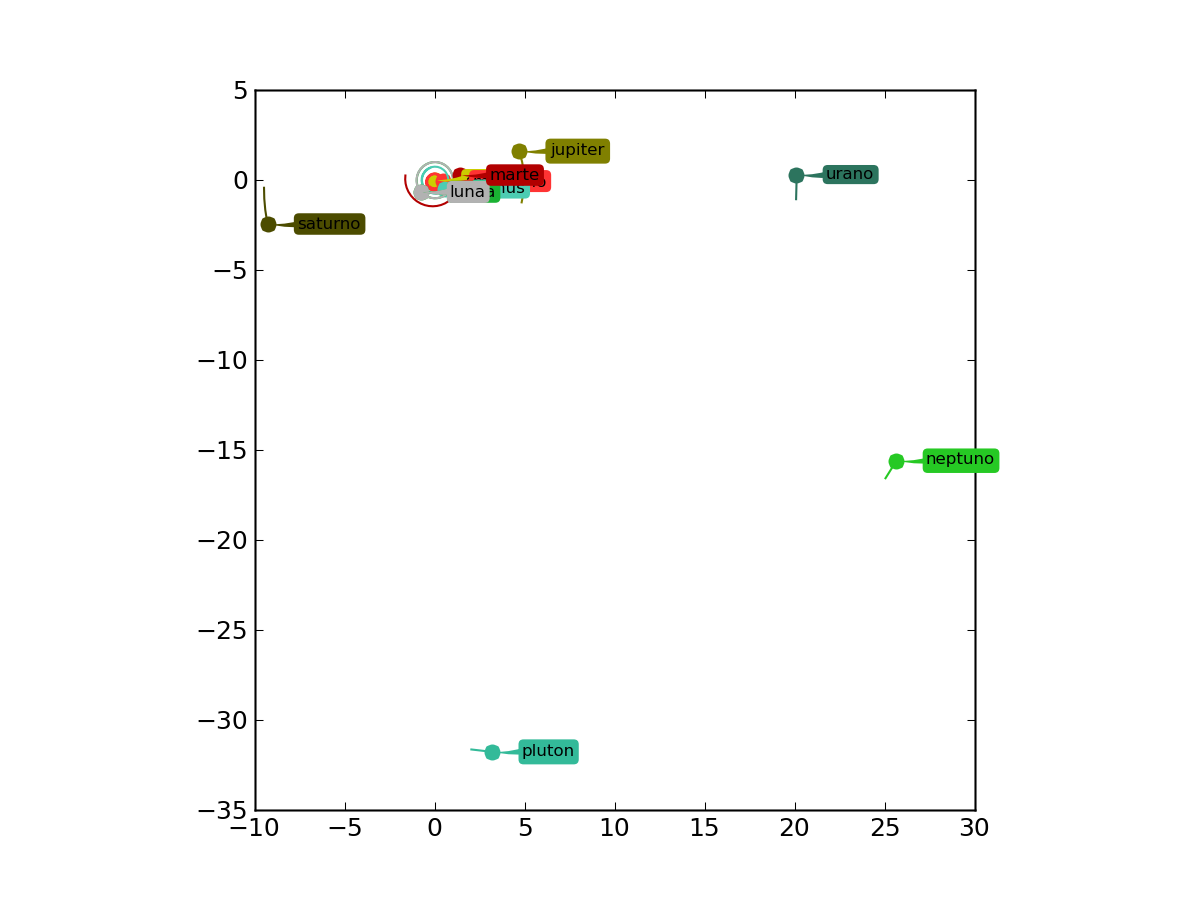
\includegraphics[scale=0.38]{img/ej2/metodo_1/validacion_365_12.png}
	\label{fig:ej2_m1_365_12}
	}
	\subfigure[$\Delta t$ = 1 hora]{
	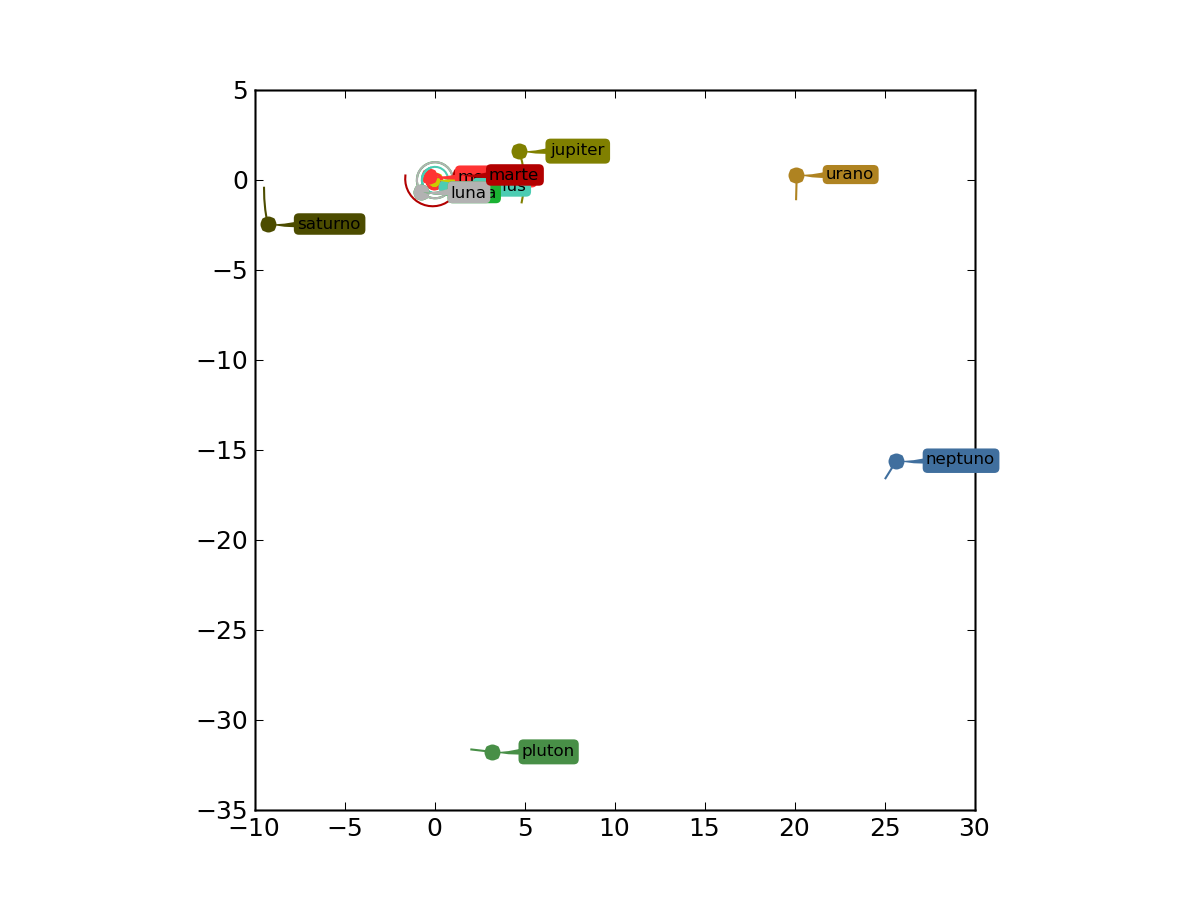
\includegraphics[scale=0.38]{img/ej2/metodo_1/validacion_365_24.png}
	\label{fig:ej2_m1_365_24}
	}
	\caption{
		Simulación de validación del sistema solar para un período de 1 año y distintos $\Delta t$
		con el método 1.
		Vemos que las órbitas de los planetas del ejercicio anterior se siguen comportando bien,
		lo que era de esperarse ya que los planetas que agregamos no deberían influenciar demasiado sus órbitas, por estar muy distanciados.
	}
	\label{ fig:res_ej2_m1_365 }
\end{figure}
\begin{figure}
	\centering
	\subfigure[$\Delta t$ = 1 día]{
	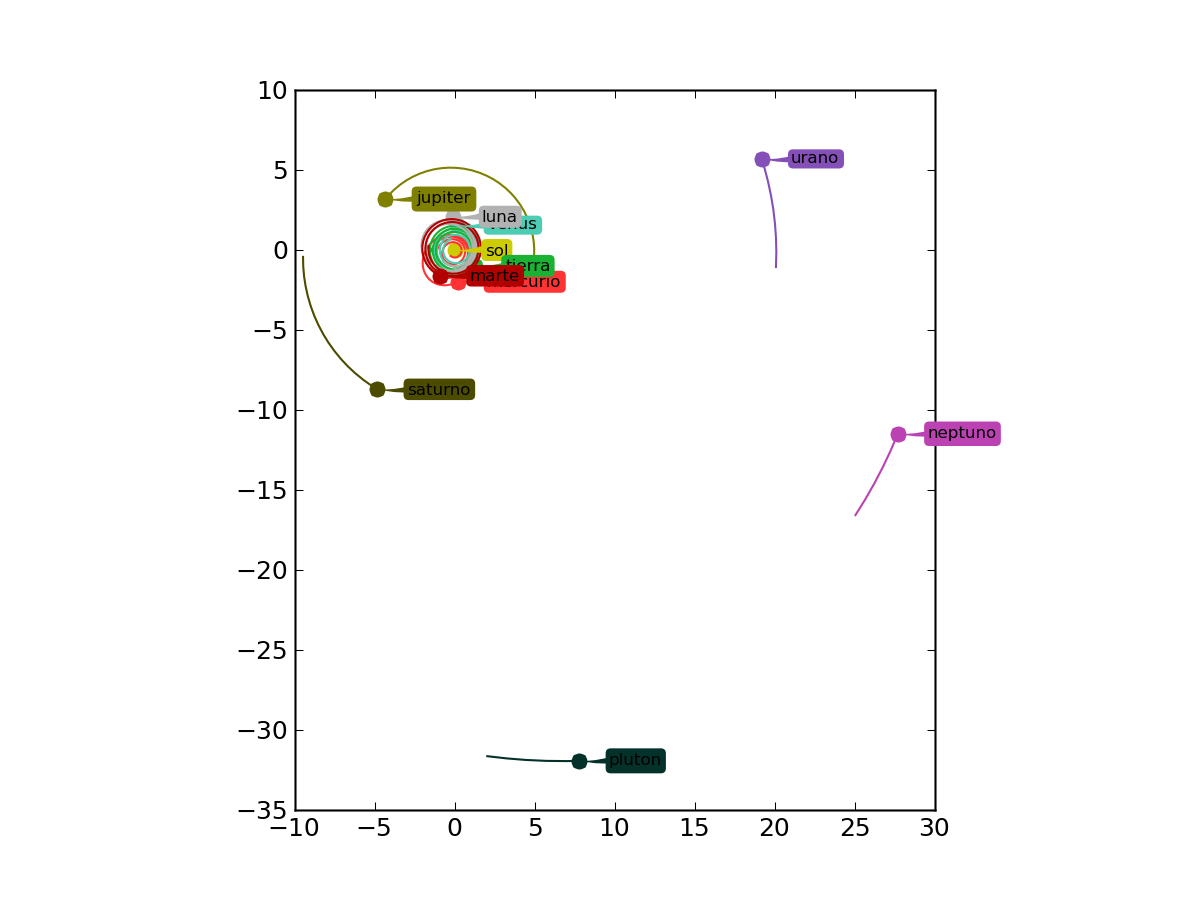
\includegraphics[scale=0.38]{img/ej2/metodo_1/validacion_1825_1.png}
	\label{fig:ej2_m1_1825_1}
	}
	\subfigure[$\Delta t$ = 6 horas]{
	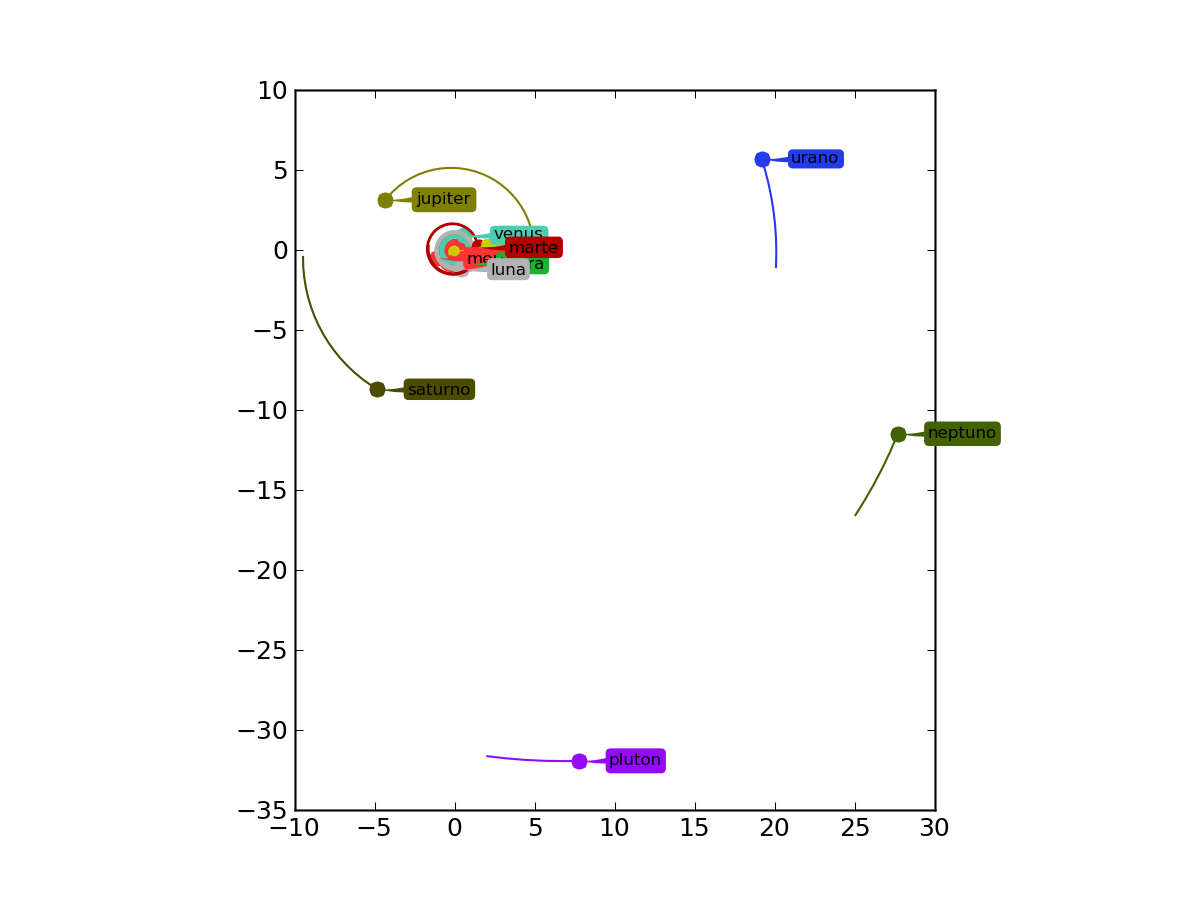
\includegraphics[scale=0.38]{img/ej2/metodo_1/validacion_1825_4.png}
	\label{fig:ej2_m1_1825_4}
	}
	\\
	\subfigure[$\Delta t$ = 2 horas]{
	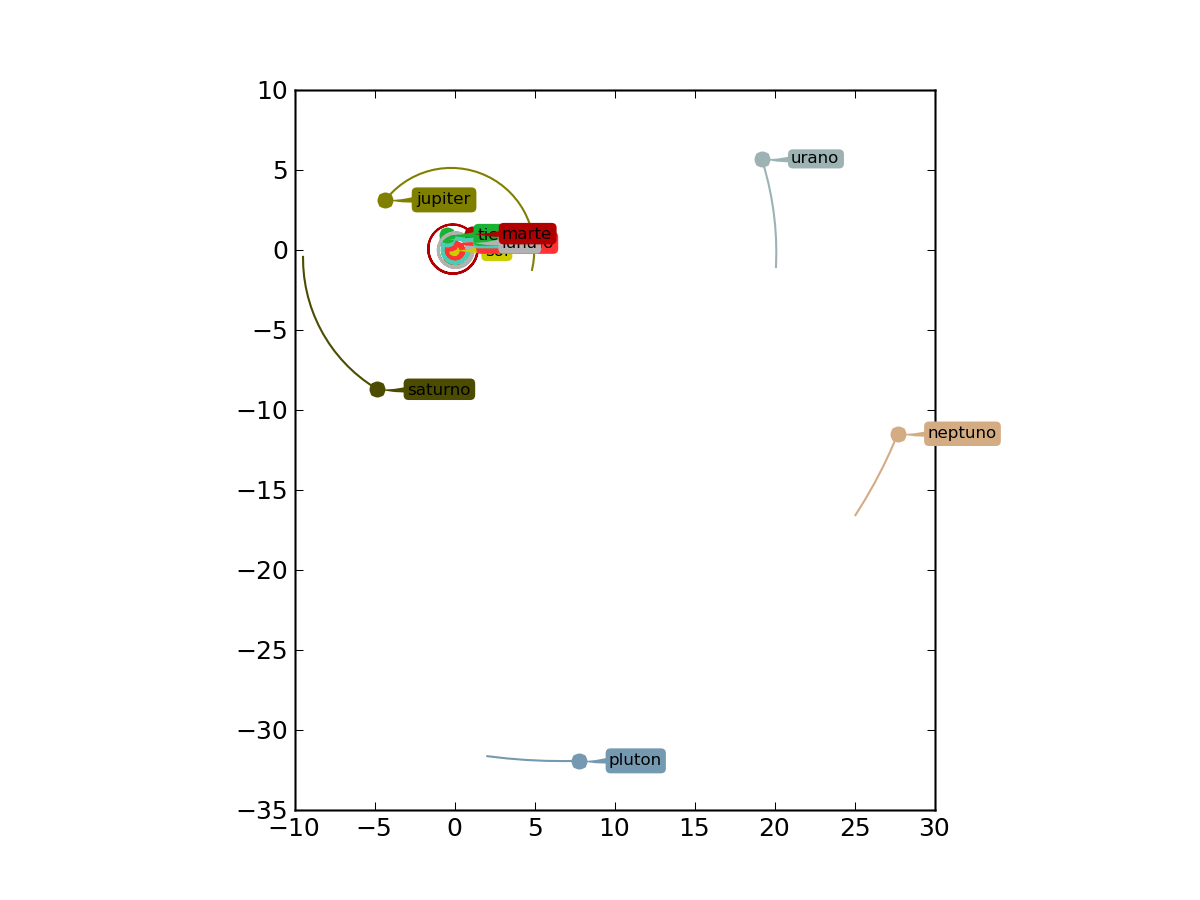
\includegraphics[scale=0.38]{img/ej2/metodo_1/validacion_1825_12.png}
	\label{fig:ej2_m1_1825_12}
	}
	\subfigure[$\Delta t$ = 1 hora]{
	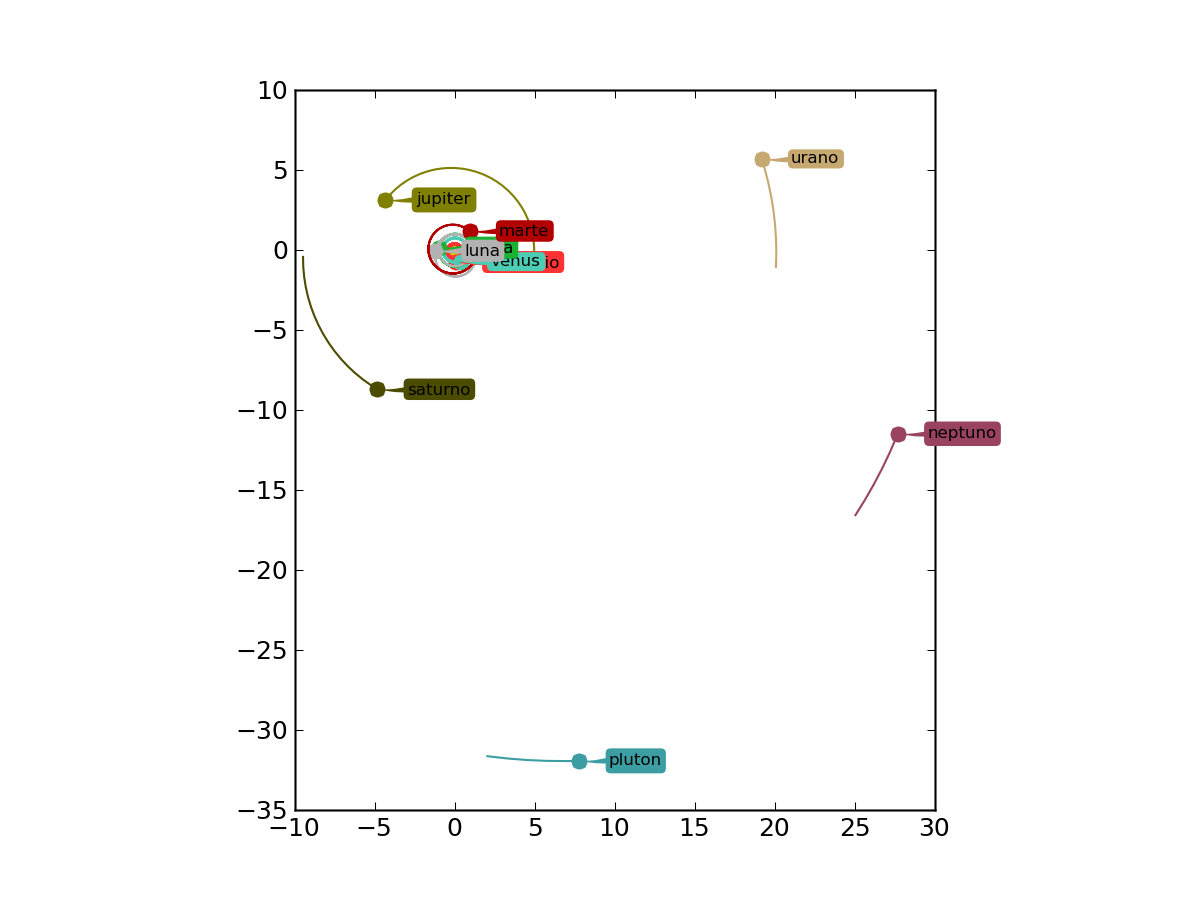
\includegraphics[scale=0.38]{img/ej2/metodo_1/validacion_1825_24.png}
	\label{fig:ej2_m1_1825_24}
	}
	\caption{
		Simulación de validación del sistema solar para un período de 5 años y distintos $\Delta t$
		con el método 1.
		No vemos cambios mayores a simple vista a esta escala,
		lo que indica que para las dimensiónes del sistema solar,
		las simulaciónes de las órbitas mas grandes son razonables también con $\Delta t$ mas chicos para este período
		(depende de que precisión se este buscando).
	}
	\label{ fig:res_ej2_m1_1825 }
\end{figure}
